% 
%% SOSP 2017 Template
%%
%% Uses sigplanconf from:
%% 
%%    http://www.sigplan.org/sites/default/files/sigplanconf.cls
%%
%% with 10pt and preprint options. 
%%
%% Replace 'XX' with your paper number (assigned when you register abstract)
%% Replace 'NN' with actual number of pages. 

\documentclass[10pt,preprint]{sigplanconf}
\usepackage{times}

\usepackage{datetime}
\usepackage{url}
\usepackage{hyperref}
\usepackage{graphicx}
\usepackage{listings}

\conferenceinfo{SOSP'17}{October 29--31, 2017, Shanghai, China}
\copyrightyear{2017} 


% These only appear when the 'preprint' option is specified.
% Enabling these will cause the first page of the document to fail the 
% format check on HotCRP :-(
%\titlebanner{Under submission to SOSP 2017 - do not cite or distribute}
%\preprintfooter{Draft of {\currenttime}, \today{}}

% No date in title area.
\date{}

% Paper number and no. of pages as author
\authorinfo{Keyan Chen(kc32),  Zhiyuan Tang(zt6)}{8 pages}


% Actual document begins below.
\begin{document}

\title{Generic Mutex Subsystem of Linux Kernel} 
\maketitle

\begin{abstract}

Sample abstract.

\end{abstract}

\section{Breif History and Background}

In the linux kernel, mutexes refer to a particular locking primitive that enforces serialization on shared memory systems, and not only to the generic term referring to ‘mutual exclusion’ found in academia or similar theoretical textbooks. \\\\
Before 2006, when developers wanted to gain mutual exclusion among their shared memory systems, they would use binary semaphores, which are sleeping locks. However, Mutexes were introduced in 2006 as an alternative to binary semaphores and this new data structure provided a number of advantages, including simpler interfaces, and at that time smaller code. 

\subsection{Why Mutex?}
Why do we need a new mutex subsystem? And what's wrong with semaphores?\\
\begin{enumerate}
	\item 'struct mutex' is smaller.
	\begin{enumerate}
		\item On x86, 'struct semaphore' is 20 bytes, 'struct mutex' is 16 bytes. A smaller structure size means less RAM footprint, and better CPU-cache utilization
	\end{enumerate}
	\item Mutex can result in tighter code
	\begin{enumerate}
		\item On x86 we can get the following .text sizes when switching all mutex-alike semaphores in the kernel to the mutex subsystem
		\begin{figure}[h!]
			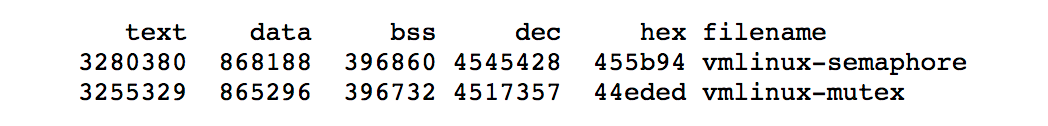
\includegraphics[scale=0.5]{image00.png}
		\end{figure}
		\item That's 25021 bytes of code saves, or a 0.76\% win off the hottest codes paths of the kernel
		\item Smaller code means better in-cache footprint, which is one of the major optimization goals in the linux kernel when people were proposing the addition of mutex subsystem in 2006. 
	\end{enumerate}
	\item The mutex subsystem is faster and has superior scalability for contented workloads.
	\begin{enumerate}
		\item On a 8-way x86 system, running a mutex based kernel and testing create+unlink+close(of separate, per-task files) in /tmp with 16 parallel tasks, the average number of ops/sec is 
		\begin{figure}[h!]
			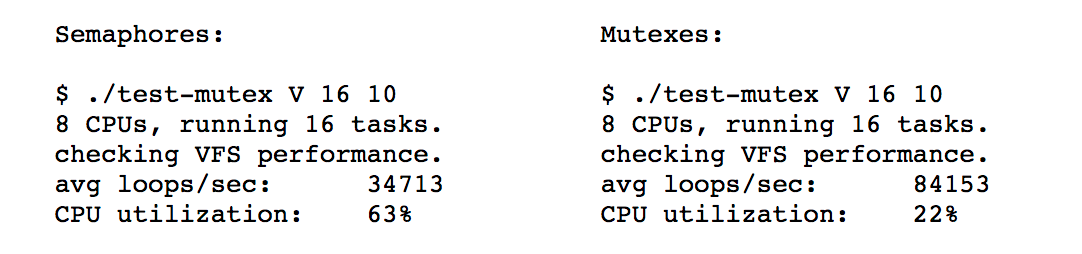
\includegraphics[scale=0.55]{image01.png}
		\end{figure}
		\item In this workload, mutex based kernel was \textbf{2.4 times} faster than the semaphore based kernel, and it also had \textbf{2.8 times} less CPU utilization. 
	\end{enumerate}
\end{enumerate}


\subsection{Design and Implementation details}
Mutex is represented by ‘struct mutex’, defined in include/linux/mutex.h and implemented in kernel/locking/mutex.c. The mutex uses a three state atomic counter to represent the different possible transitions that can occur during the lifetime of a mutex:
\begin{itemize}
	\item 1: unlocked
	\item 0: locked, no waiters
	\item negative: locked, with potential waiters
\end{itemize}
In its most basic form it also includes a wait-queue and a spinlock that serializes access to it. When acquring a mutex, there are three possible paths that can be taken, depending on the state of lock:
\begin{enumerate}
	\item Fastpath: tries to atomically acquire the lock by decrementing the counter. If it was already taken by another task it goes to the next possible path. This logic is architecture specific.
	\item Mid-path: aka optimistic spinning. It tries to spin for acquisition while the lock owner is running and there are no other tasks ready to run that have higher priority. The rationale is that if the lock owner is running, it is likely to release the lock soon. The mutex spinners are queued up using MCS lock so that only one spinner can compete for the mutex. The MCS lock is a simple spinlock with the desirable properties of being fair and with each cpu trying to acquire the lock spinning on a local variable. It avoids expensive cache-line bouncing that common test-and-set spinlock implementations incur. And MCS-like lock is specially tailored for optimistic spinning for sleeping lock implementation.
	\item Slowpath: last resort, if the lock is still unable to be acquired, the task is added to the wait-queue and sleeps until woken up by the unlock path. Under normal circumstances it blocks as TASK\_UNINTERRUPTIBLE.
\end{enumerate}

\newpage

\section{Interesting Findings}
\subsection{Unique Optimistic Spinning in Linux Mutex Subsystem}
While formally kernel mutexes are sleepable locks, it is the Mid-path(aka optimistic spinning) that makes the mutex subsystem now more practically a hybrid type. By simply not interrupting a task and busy-waiting for a few cycles instead of immediately sleeping, the performance of this lock has been seen to significantly improve a number of workloads. \\

\begin{figure}[h!]
	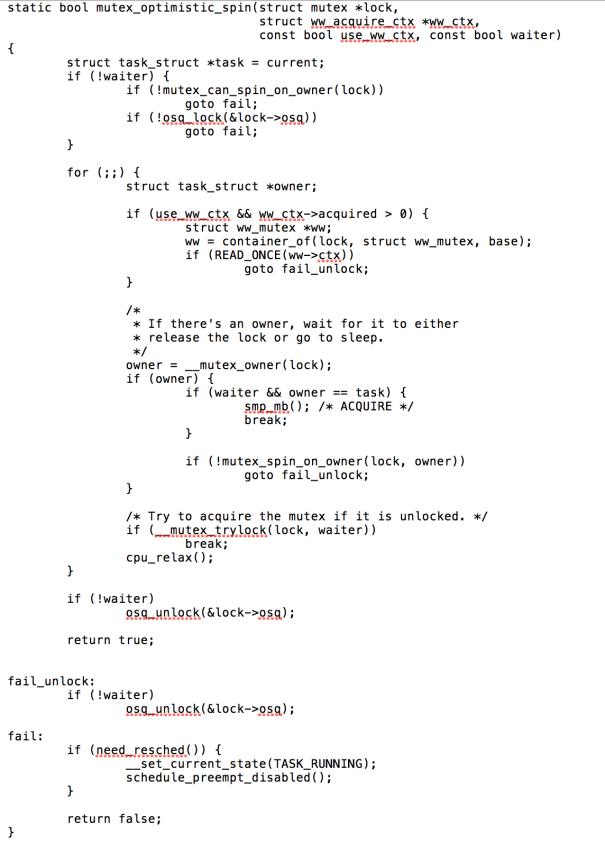
\includegraphics[scale=1]{image02.png}
	\caption{Use of MCS and the Optimistic Spinning routine in the source code}
\end{figure}

\newpage
\subsection{Design and Use of MCS locks in linux kernel}
In mutex subsystem, mutex spinners are queued up using MCS locks as talked about above. 
The design of MCS lock and the difference between MCS lock and ordinary spinlock is also a very interesting design decision in linux kernel.\\
The concept of a spinlock is simple and straight-forward. When a thread wants to acquire the lock it will attempt to set the lock bit of that spinlock with an atomic compare-and-swap(CAS) instruction and repeatedly spin there in the lock can not be acquired during one CAS. \\
However, spinlocks have some fundamental problems. One of those is that every attemp to acquire a lock requires moving the cache line containing that lock to the local CPU. This cache-line bouncing can be extremely bad to performance for contended locks. Therefore, developers had been working on reducing the cache contention of spinlocks and thus, MCS locks were introduced by Tim Chen to solve this problem.\\
The structure of MCS lock is defined in struct mcs\_spinlock\\
\begin{figure}[h!]
	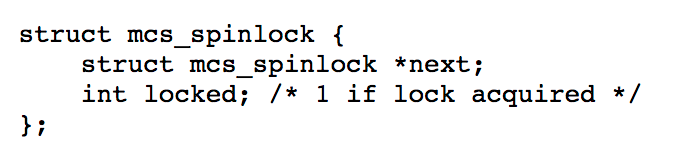
\includegraphics[scale=0.8]{mcslock0.png}
\end{figure}\\
Here we will go step-by-step to demonstrate how a MCS lock works and thus, we can see the difference between MCS lock and ordinary spinlock, as well as why MCS lock is guaranteed to provide a FIFO ordering on unlocking waiting threads. \\

\begin{itemize}
	\item From mcs\_spinlock we can visualize an unlocked MCS lock as the following:\\
	\begin{figure}[h]
		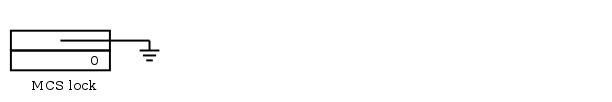
\includegraphics[scale=0.4]{mcslock1.png}
	\end{figure}\\
	\item Now when a new CPU thread is going to acquire the MCS lock, it will instantiate a mcs\_spinlock structure on its own thread and use an unconditional atomic exchange operation to try to store the address of its own mcs\_spinlock in the next field of the main MCS lock. The atomic exchange will return the previous value of the main MCS lock's next field. In this case when the previous next value of null pointer is returned back to the CPU thread acquiring the lock, it will know that is successfully acquires the lock. At this point the system can be visualized in this figure:\\
	\begin{figure}[h!]
		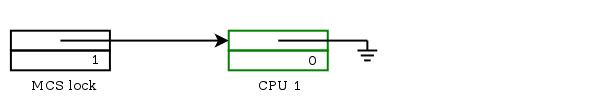
\includegraphics[scale=0.4]{mcslock2.png}
	\end{figure}\\
	\item Most interesting thing comes to our view when a second CPU thread is going to acquire the same MCS lock. If there's a second CPU thread trying to acquire the MCS lock while the lock hasn't been unlocked yet, the thread will still try the same locking routine as specified above. And then the returned mcs\_spinlock address from the atomic swap will be a pointer to the first CPU thread's mcs\_spinlock structure. In this case the second CPU will know that it doesn't acquire the MCS lock and will thus, store a pointer to its own mcs\_spinlock structure in the next field of the first CPU thread's mcs\_spinlock structure. The system at this point can be visualized in this figure:
	\begin{figure}[h!]
		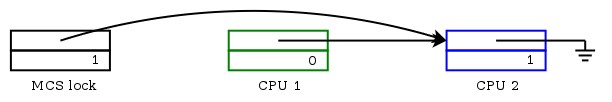
\includegraphics[scale=0.33]{mcslock4.png}
	\end{figure}\\
	\item Once this assignment is done, the second CPU thread will spin on the locked value in its own mcs\_spinlock structure rather than the locked value in the main MCS lock's structure. Therefore, the second CPU thread's spinning will be entirely CPU-local. As more CPU threads are joining this waiting queue, each thread will be spinning on the locked value of its local mcs\_spinlock structure and form a chain of waiting queue, which by its structure, guarantees a FIFO unlock ordering. 
	\item Finally when the first CPU thread is going to unlock the MCS lock, it will first try to do a compare-and-swap(CAS) operation on the main MCS lock's next field to set it to null pointer under the assumption that the next field still points to itself. In that CAS operation fails, the first thread will know that there are other waiting threads and thus, find the mcs\_spinlock structure of the second thread and change its locked value in order to stop second thread from spinning and unlock it. The system at this point can be visualized in this figure:
	\begin{figure}[h!]
		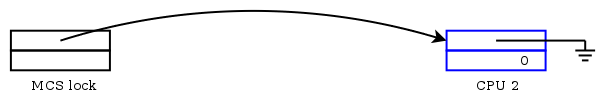
\includegraphics[scale=0.3]{mcslock5.png}
	\end{figure}
	
	
In conclusion, an MCS lock is more complicated than a ordinary spinlock. But the added complexity removes much of the cache-line bouncing in ordinary spinlock and ensures unlocking fairness. Therefore, mutex subsystem in linux kernel chooses to use MCS locks to queue up mutex spinners. 
\end{itemize}

\newpage
\subsection{Bug in an obviously correct reference count code pattern}
This bug comes from a kernel crash reported in July 2013. And this bug report had not been resolved until December 2013. And people found out surprisingly that an "obviously correct" reference count code pattern turns out to have potential data race problems that can lead to dangerous bugs. And understanding this bug requires a deep understanding about linux kernel mutex subsystem, especially its unique optimistic spinning phase. Before going deep into the analysis of the bug, let's first see a piece of code, which manipulates a structure called "s" and this structure is protected by a mutex embedded with it. 
\lstset{language=C}
\begin{lstlisting}
int free = 0;

mutex_lock(&s->lock);
if (--s->refcount == 0) {
	free = 1;
}

mutex_unlock(&s->lock);
if (free) {
	kfree(s);
}

\end{lstlisting}
From a first look, this piece of code just "works". It simply locks s, decrements reference counter to s, detects whether we can free s, and then unlock s. However, because of the fact that current implementation of mutex has an optimistic spinning phase while acquiring the lock, this piece of code is no longer data race free. \\
The structure mutex has an atomic counter and a spinlock. When the lock is free and one thread is going to acquire lock, it will atomically decrement the counter to 0 and continue, which is known as the fast path as specified in section 1.2.\\
And when the thread is going to unlock mutex, it will atomically increment counter to 1 if counter is 0, which means that there are no waiting threads on this mutex currently. If the current value of counter is negative, the mutex\_unlock() routine need to also wake up the first waiting thread on mutex. In code the lifecycle of a mutex can be shown as below.
\begin{lstlisting}
spin_lock(&lock->wait_lock);
atomic_set(&lock->count, 1);
// wake up first waiting thread
wake_up_process(); 
spin_unlock(&lock->wait_lock);
\end{lstlisting}
At this point the bug gradually becomes clear to us. Because of the optimistic spinning phase, a newly coming thread which is currently doing optimistic spinning will immediately take the lock once it sees the effect of 
\begin{lstlisting}
atomic_set(&lock->count, 1);
\end{lstlisting}
Therefore, when the original owner of lock is calling 
\begin{lstlisting}
wake_up_process(); 
\end{lstlisting}
to wake up the next waiting thread, a newly coming thread already believes that it takes the lock and if this newly coming thread quickly frees the data structure containing the lock, the final 
\begin{lstlisting}
spin_unlock(&lock->wait_lock);
\end{lstlisting}
will be applied to already freed memory space, and thus causing all sorts of problems. \\
Therefore, Linus Torvalds, the finder of this concurrency bug, concludes:\\

\textit{In other words, it's unsafe to protect reference counts inside objects with anything but spinlocks and/or atomic refcounts. Or you have to have the lock "outside" the object you're protecting(which is often what you want for other reasons anyway, notably lookup)}\\


\bibliographystyle{acm}
% \bibliography{xxx}

\end{document}
